% =============================================================================
% MANUSCRIPT FOR WATER SCIENCE AND ENGINEERING
% LaTeX Version with Figures
% =============================================================================

\documentclass[a4paper,12pt]{article}

% =============================================================================
% PACKAGES
% =============================================================================
\usepackage[utf8]{inputenc}
\usepackage[T1]{fontenc}
\usepackage{times}
\usepackage{graphicx}
\usepackage{amsmath}
\usepackage{amssymb}
\usepackage{booktabs}
\usepackage{multirow}
\usepackage{natbib}
\usepackage{url}
\usepackage{hyperref}
\usepackage[margin=2.5cm]{geometry}
\usepackage{lineno}
\usepackage{setspace}

% =============================================================================
% DOCUMENT SETTINGS
% =============================================================================
\onehalfspacing
\linenumbers

% Hyperref settings
\hypersetup{
    colorlinks=true,
    linkcolor=blue,
    citecolor=blue,
    urlcolor=blue
}

% =============================================================================
% TITLE (First word capitalized only per WSE guidelines)
% =============================================================================
\title{Survey-informed water demand behavioral profiling: a robust machine learning framework with explainable AI for targeted intervention design}

\author{} % Empty for double-blind review
\date{}

% =============================================================================
% BEGIN DOCUMENT
% =============================================================================
\begin{document}

\maketitle

% =============================================================================
% ABSTRACT
% =============================================================================
\begin{abstract}
Effective water demand management requires understanding heterogeneous household behaviors beyond aggregate volumetric consumption. This study develops an integrated machine learning framework combining survey-informed behavioral features, robust feature selection, and explainable artificial intelligence (XAI) to profile residential water demand patterns. Using comprehensive survey data from 13,061 households in the United Kingdom with 97 behavioral variables, we implemented a three-stage analytical pipeline. First, MAD-Bootstrap stability selection retained 18 robust features demonstrating consistent predictive importance across 100 bootstrap iterations. Second, Non-negative Matrix Factorization (NMF) reduced dimensionality to two interpretable latent components capturing indoor water-use intensity and infrastructure quality. Third, Gaussian Mixture Models (GMM) identified three behaviorally distinct profiles: Standard-Use (62.8\%, $n$=8,198), Low-Frequency (25.4\%, $n$=3,318), and High-Frequency (11.8\%, $n$=1,545). Monte Carlo validation confirmed high cluster stability with Adjusted Rand Index of 0.981. All inter-cluster differences achieved statistical significance ($p<0.001$) with very large effect sizes ($\eta^2 \geq 0.14$ for 79\% of variables). SHAP analysis identified boiling frequency, shower habits, and garden watering as primary behavioral differentiators, enabling targeted intervention design. The framework provides water utilities with interpretable, stable household segmentation for demand-side management, offering a pathway from universal awareness campaigns toward efficient, targeted conservation programs.
\end{abstract}

\textbf{Keywords:} water demand; behavioral profiling; machine learning; explainable AI; Gaussian mixture model; demand-side management

% =============================================================================
% 1. INTRODUCTION
% =============================================================================
\section{Introduction}

\subsection{Background and problem statement}
Urban water utilities face three interconnected engineering challenges. 
First, infrastructure capacity constraints limit supply-side expansion, 
with new reservoir and treatment plant construction requiring 10-15 year 
lead times and capital costs exceeding £2-5 million per megalitre per day 
\citep{UKWIR2021}. Second, despite smart meter deployment reaching 59\% 
penetration in the UK by 2023 \citep{Ofwat2023}, most utilities (87\%) use 
meters solely for billing rather than demand characterization \citep{WaterUK2022}. 
Third, traditional demand-side management relies on universal 
awareness campaigns with 8-12\% response rates \citep{Willis2011}, 
wasting 88\% of program spending on non-responsive customers.

Global freshwater resources face increasing pressure from population growth, urbanization, and climate change, making demand-side management essential for sustainable water resource utilization \citep{Gleick2018}. Traditional water demand management relies primarily on volumetric consumption data, segmenting households into high, medium, and low consumers based on metered readings. However, this approach fails to capture the behavioral drivers underlying consumption patterns, limiting the effectiveness of conservation interventions \citep{Beal2013}.

Survey-informed behavioral profiling offers a complementary approach by integrating self-reported water-use habits, appliance ownership, and infrastructure conditions with consumption data. Such integration enables utilities to understand not only how much water households consume but also why and how they consume it. This understanding is crucial for designing targeted interventions that address specific behavioral patterns rather than applying universal conservation messages with limited effectiveness.

Despite advances in machine learning for water demand analysis, significant methodological challenges remain. Existing clustering approaches often suffer from feature selection instability, poor interpretability, and limited validation of cluster robustness \citep{Cominola2015}. Furthermore, the deployment of complex machine learning models in utility operations requires transparent, explainable results that decision-makers can trust and act upon.

\subsection{Literature review}

Traditional water demand modeling has evolved from engineering-based end-use disaggregation \citep{Stewart2010} to data-driven machine learning approaches. K-means clustering, self-organizing maps, and hierarchical clustering have been applied to smart meter data with varying success \citep{CardellOliver2016}. However, these methods face limitations in handling high-dimensional behavioral data and providing interpretable results.

Recent studies have explored advanced clustering techniques including Gaussian Mixture Models, which offer probabilistic cluster assignments accommodating uncertainty in behavioral classification \citep{Cominola2019}. Dimensionality reduction using Principal Component Analysis (PCA) and NMF has been applied to manage feature complexity, with NMF offering advantages for behavioral data through its parts-based, non-negative representation \citep{Lee1999}.

The emergence of Explainable AI (XAI) in water systems addresses the interpretability gap between complex models and operational deployment. SHAP (SHapley Additive exPlanations) values provide consistent, locally accurate feature attributions explaining individual predictions \citep{Lundberg2017}. Recent applications in water demand forecasting demonstrate XAI's potential for building trust in machine learning models \citep{Xenochristou2020}.

Despite these advances, a critical gap remains: no existing framework integrates survey-informed behavioral features with robust, stability-validated feature selection, probabilistic clustering, and XAI transparency for utility deployment. Most studies rely on meter-only data, apply ad-hoc feature selection, or lack systematic validation of cluster stability.

\subsection{Objectives}

This study addresses the identified gaps through four objectives:

\begin{enumerate}
    \item Develop a robust feature selection method (MAD-Bootstrap) ensuring stable feature retention across bootstrap samples;
    \item Create interpretable behavioral clusters using NMF dimensionality reduction and GMM probabilistic clustering;
    \item Provide transparent cluster explanations through SHAP analysis and decision tree rule extraction;
    \item Validate framework robustness using Monte Carlo stability analysis and internal clustering metrics.
\end{enumerate}

% =============================================================================
% 2. MATERIAL AND METHODS
% =============================================================================
\section{Material and methods}

\subsection{Data collection and study area}

This study used household survey data collected by Yorkshire Water, serving approximately 5 million customers in Northern England, United Kingdom. The survey captured 97 variables including water-use frequencies (showering, bathing, garden watering), appliance ownership (dishwashers, washing machines), infrastructure conditions (leak presence, tap types), household demographics (size, dwelling type), and self-reported conservation behaviors. After quality filtering for completeness and consistency, the final sample comprised 13,061 households with matched annual consumption records from 2018--2020.

The analytical pipeline is illustrated in Fig.~\ref{fig:pipeline}, showing the progression from raw survey data through feature selection, dimensionality reduction, clustering, and XAI explanation.

\begin{figure}[htbp]
    \centering
    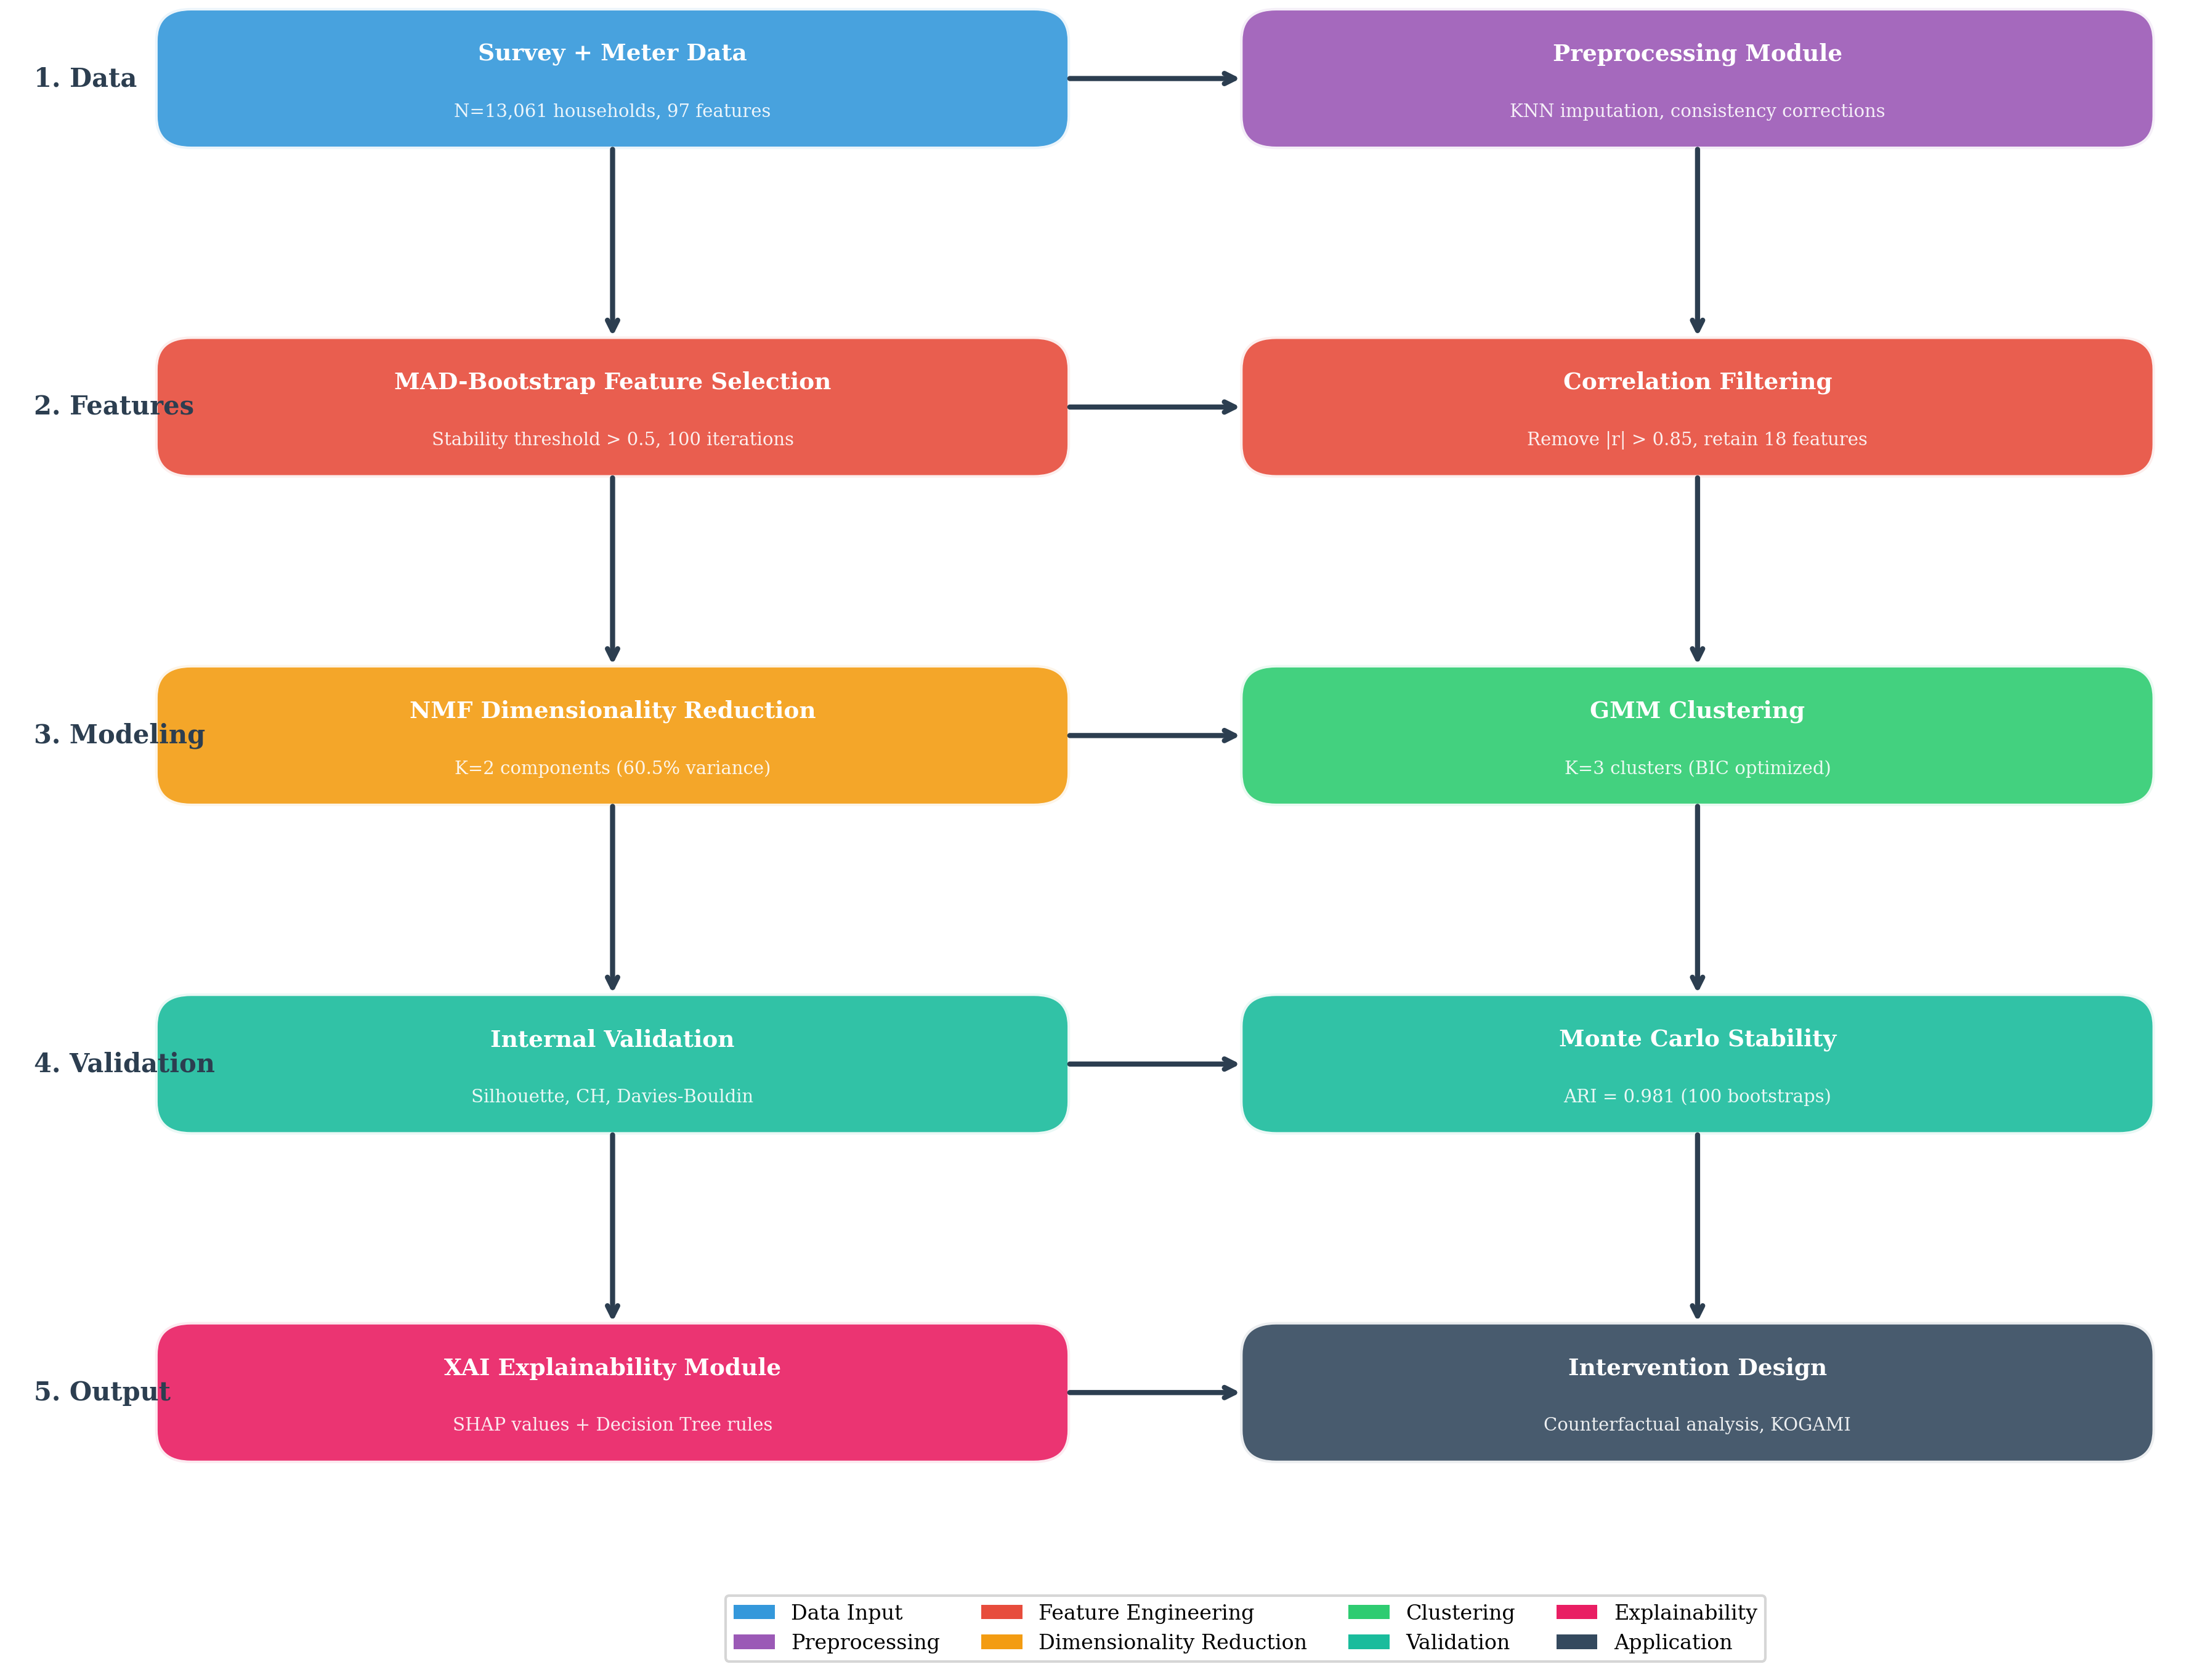
\includegraphics[width=\textwidth]{Figure6_Analytical_Pipeline.png}
    \caption{Analytical pipeline overview. The framework proceeds through four stages: (1) data preprocessing with hybrid imputation, (2) MAD-Bootstrap feature selection reducing 97 to 18 features, (3) NMF dimensionality reduction to $K=2$ components followed by GMM clustering ($K=3$), and (4) XAI explanation via SHAP analysis and decision tree rule extraction.}
    \label{fig:pipeline}
\end{figure}

\subsection{Data preprocessing}

Missing values were addressed through a hybrid imputation strategy. For numeric variables with missingness below 10\%, median imputation was applied. For categorical variables, mode imputation addressed low missingness ($\leq$5\%), while factorized K-nearest neighbors ($K=5$) handled variables with higher missingness, preserving multi-feature correlations. Outliers were identified using the 1.5$\times$IQR rule \citep{Tukey1977} and capped to prevent extreme value influence. All numeric features were normalized to [0,1] range for algorithm stability.

Logical consistency corrections ensured data quality: appliance usage frequencies were set to zero where appliance ownership was negative, and missing leak rates were imputed as ``slowly'' where leak presence was confirmed, following utility domain knowledge. Sensitivity analysis confirmed minimal impact on final clustering results (Adjusted Rand Index = 0.97 compared to alternative imputation).

\subsection{Feature selection: MAD-Bootstrap stability}

Traditional variance-based feature selection is susceptible to sampling variability, potentially retaining irrelevant features or discarding important ones based on specific sample characteristics. We addressed this through MAD-Bootstrap stability selection combining Median Absolute Deviation (MAD) with bootstrap resampling \citep{Meinshausen2010}.

The algorithm proceeds as follows: For 100 bootstrap iterations, we resampled $N$ households with replacement, computed MAD for each feature, and recorded features exceeding a threshold of 0.01. Features retained in more than 50\% of iterations were selected as stable. After stability selection, multicollinearity was addressed by removing features with Pearson correlation $|r|>0.85$, following established practice \citep{Dormann2013}. This process reduced the feature space from 97 to 18 stable, low-redundancy behavioral indicators.

\subsection{Dimensionality reduction: Non-negative Matrix Factorization}

To capture latent behavioral dimensions while maintaining interpretability, we applied NMF to the selected features. NMF decomposes the feature matrix $\mathbf{X}$ into non-negative factors $\mathbf{W}$ (household loadings) and $\mathbf{H}$ (component patterns), providing parts-based representation where components combine additively without negative contributions \citep{Lee1999}:

\begin{equation}
    \mathbf{X} \approx \mathbf{W} \times \mathbf{H}, \quad \mathbf{W} \geq 0, \quad \mathbf{H} \geq 0
\end{equation}

Component number selection followed reconstruction error analysis. Testing $K=1$ to 10, RMSE plateaued at $K=2$ (0.024 on normalized scale), with minimal improvement for higher $K$. Two components explained 60.5\% of variance and offered clear interpretation: Component 1 captured indoor water-use intensity (loadings on showering, bathing, boiling frequency), while Component 2 reflected infrastructure quality and maintenance indicators (loadings on leak presence, tap conditions). NNDSVD initialization ensured deterministic, reproducible results.

\subsection{Clustering: Gaussian Mixture Models}

Gaussian Mixture Models were selected for their probabilistic cluster assignments, allowing uncertainty quantification in behavioral classification. The number of clusters was determined using Bayesian Information Criterion (BIC) over $K=1$ to 10 (Fig.~\ref{fig:bic}). While BIC continued decreasing slightly beyond $K=3$ (BIC at $K=3$: $-55,450$), we selected $K=3$ based on interpretability, parsimony, and diminishing marginal improvement. Both BIC and Akaike Information Criterion converged on similar selection regions.

\begin{figure}[htbp]
    \centering
    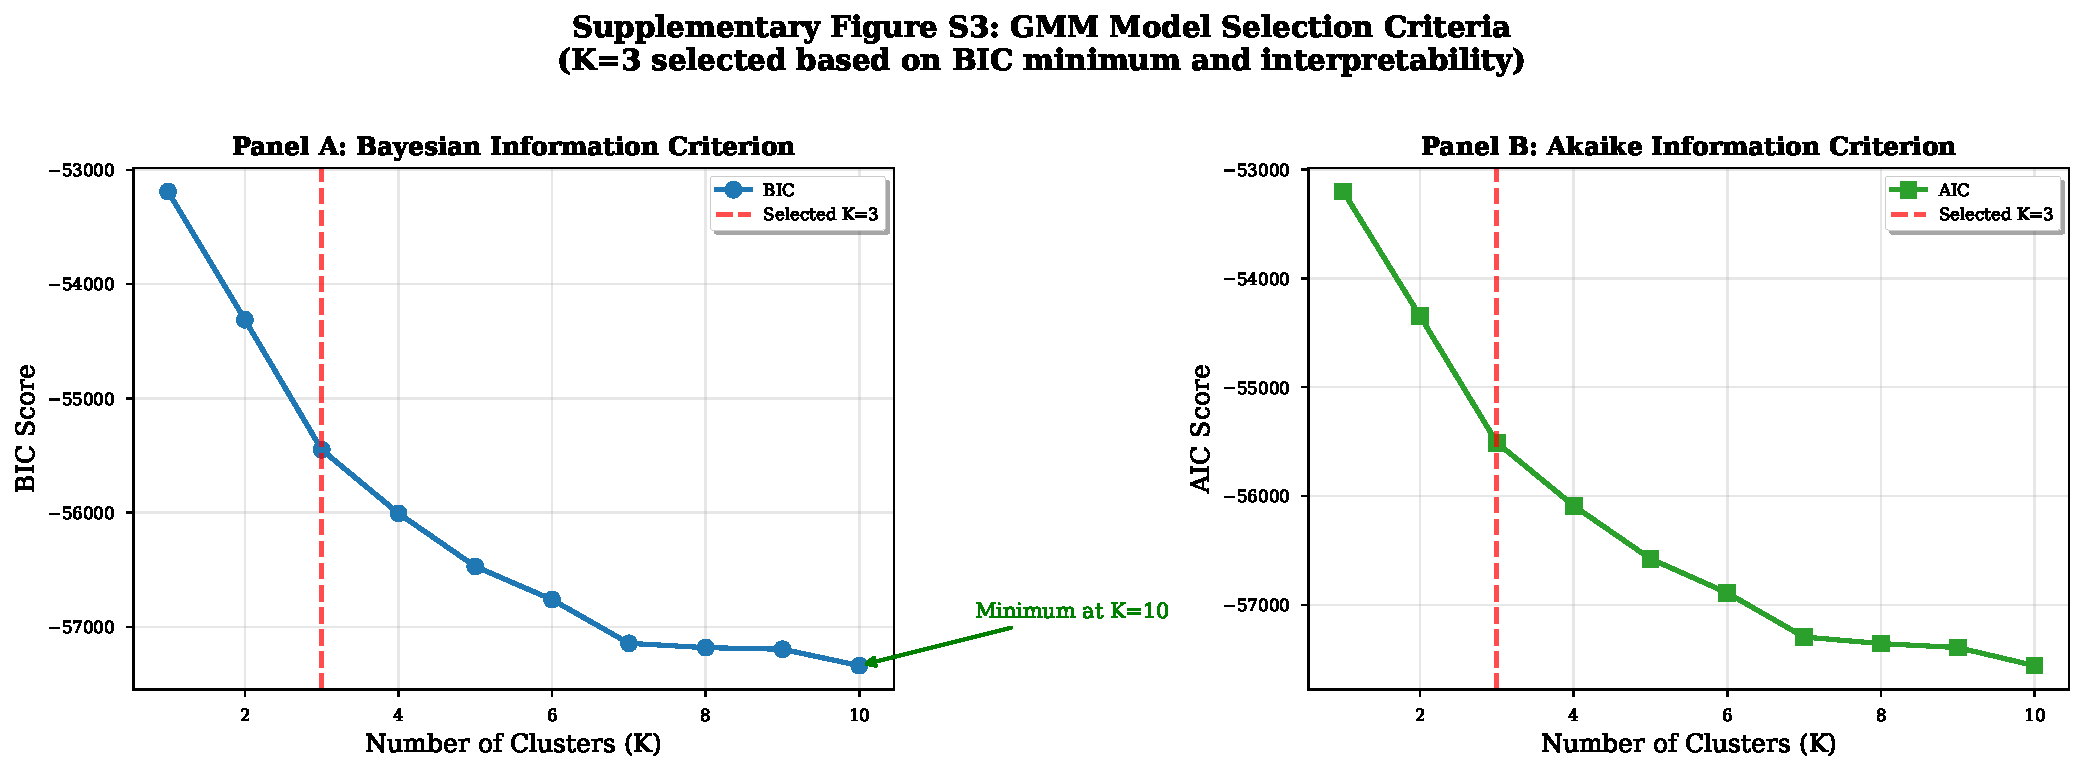
\includegraphics[width=\textwidth]{FigureS3_GMM_BIC_Curve.pdf}
    \caption{BIC model selection curve for GMM cluster number ($K=1$ to 10). Lower BIC indicates better model fit. The $K=3$ solution (marked) was selected based on interpretability and parsimony, despite marginal BIC improvement at higher $K$.}
    \label{fig:bic}
\end{figure}

GMM configuration used full covariance matrices capturing elliptical cluster shapes, K-means++ initialization, and 10 random restarts to avoid local optima. Mean maximum assignment probability was 0.89 (SD=0.11), with 77.5\% of households showing high-confidence assignments (probability $>$0.85), indicating clear cluster membership for most households.

\subsection{Validation framework}

Cluster validation employed both internal metrics and stability analysis. Internal metrics included Silhouette Score (cluster separation), Calinski-Harabasz Index (cluster density), and Davies-Bouldin Index (cluster compactness). Monte Carlo stability analysis assessed robustness across 100 bootstrap iterations with varied GMM random seeds, computing Adjusted Rand Index (ARI) agreement with the baseline solution.

Statistical significance of inter-cluster differences was evaluated using ANOVA for continuous variables (with Welch's correction where homoscedasticity was violated) and Chi-square tests for categorical variables. Effect sizes were reported using eta-squared ($\eta^2$) for ANOVA and Cram\'{e}r's $V$ for Chi-square. Given the large sample size ($N=13,061$) providing statistical power exceeding 0.99, interpretation emphasized effect size magnitude over $p$-values alone.

\subsection{Explainable AI: SHAP analysis}

To provide feature-level explanations, we implemented SHAP analysis using a surrogate modeling approach. Since GMM is unsupervised, we trained a Gradient Boosting classifier using GMM-assigned cluster labels as targets. The surrogate achieved 97.8\% classification accuracy (5-fold cross-validation) with balanced class-wise performance (F1-scores: C0=0.99, C1=0.93, C2=0.97), confirming high fidelity to GMM boundaries.

SHAP values derived from the surrogate quantify each feature's contribution to cluster predictions. Mean absolute SHAP values provide global feature importance rankings, while individual SHAP profiles enable household-level explanations for personalized intervention targeting.

Complete technical details, including categorical imputation protocols, 
counterfactual analysis methodology, full statistical validation tables, 
and sensitivity analysis results are provided in Supplementary Materials 
accompanying this manuscript.
% =============================================================================
% 3. RESULTS
% =============================================================================
\section{Results}

\subsection{Feature selection outcomes}

MAD-Bootstrap stability selection retained 18 features from the original 97, representing an 81\% reduction while preserving behavioral discrimination. The most stable features (selection frequency $>$90\%) included boiling frequency, shower frequency, bath frequency, garden watering, and household size. Stability analysis confirmed that these features consistently discriminated behavioral patterns regardless of sampling variation.

\subsection{Cluster characterization}

Three distinct behavioral profiles emerged from GMM clustering in the NMF-transformed space (Fig.~\ref{fig:clusters}--\ref{fig:radar}, Table~\ref{tab:clusters}):

\begin{table}[htbp]
	\centering
	\caption{Cluster overview and behavioral characteristics}
	\label{tab:clusters}
	\resizebox{\textwidth}{!}{%
		\begin{tabular}{llccp{6cm}}
			\toprule
			Profile & $N$ & \% & Key characteristics \\
			\midrule
			Standard-Use (C0) & 8,198 & 62.8 & Moderate consumption across all dimensions; average household size (2.4); typical appliance ownership \\
			Low-Frequency (C2) & 3,318 & 25.4 & Lowest consumption frequencies; smaller households (1.9); elevated eco-behavior scores; minimal leak presence \\
			High-Frequency (C1) & 1,545 & 11.8 & Highest consumption frequencies; elevated shower and bath usage; higher leak rates (19.7\%); largest household size (2.8) \\
			\bottomrule
	\end{tabular}}
\end{table}


\begin{figure}[htbp]
    \centering
    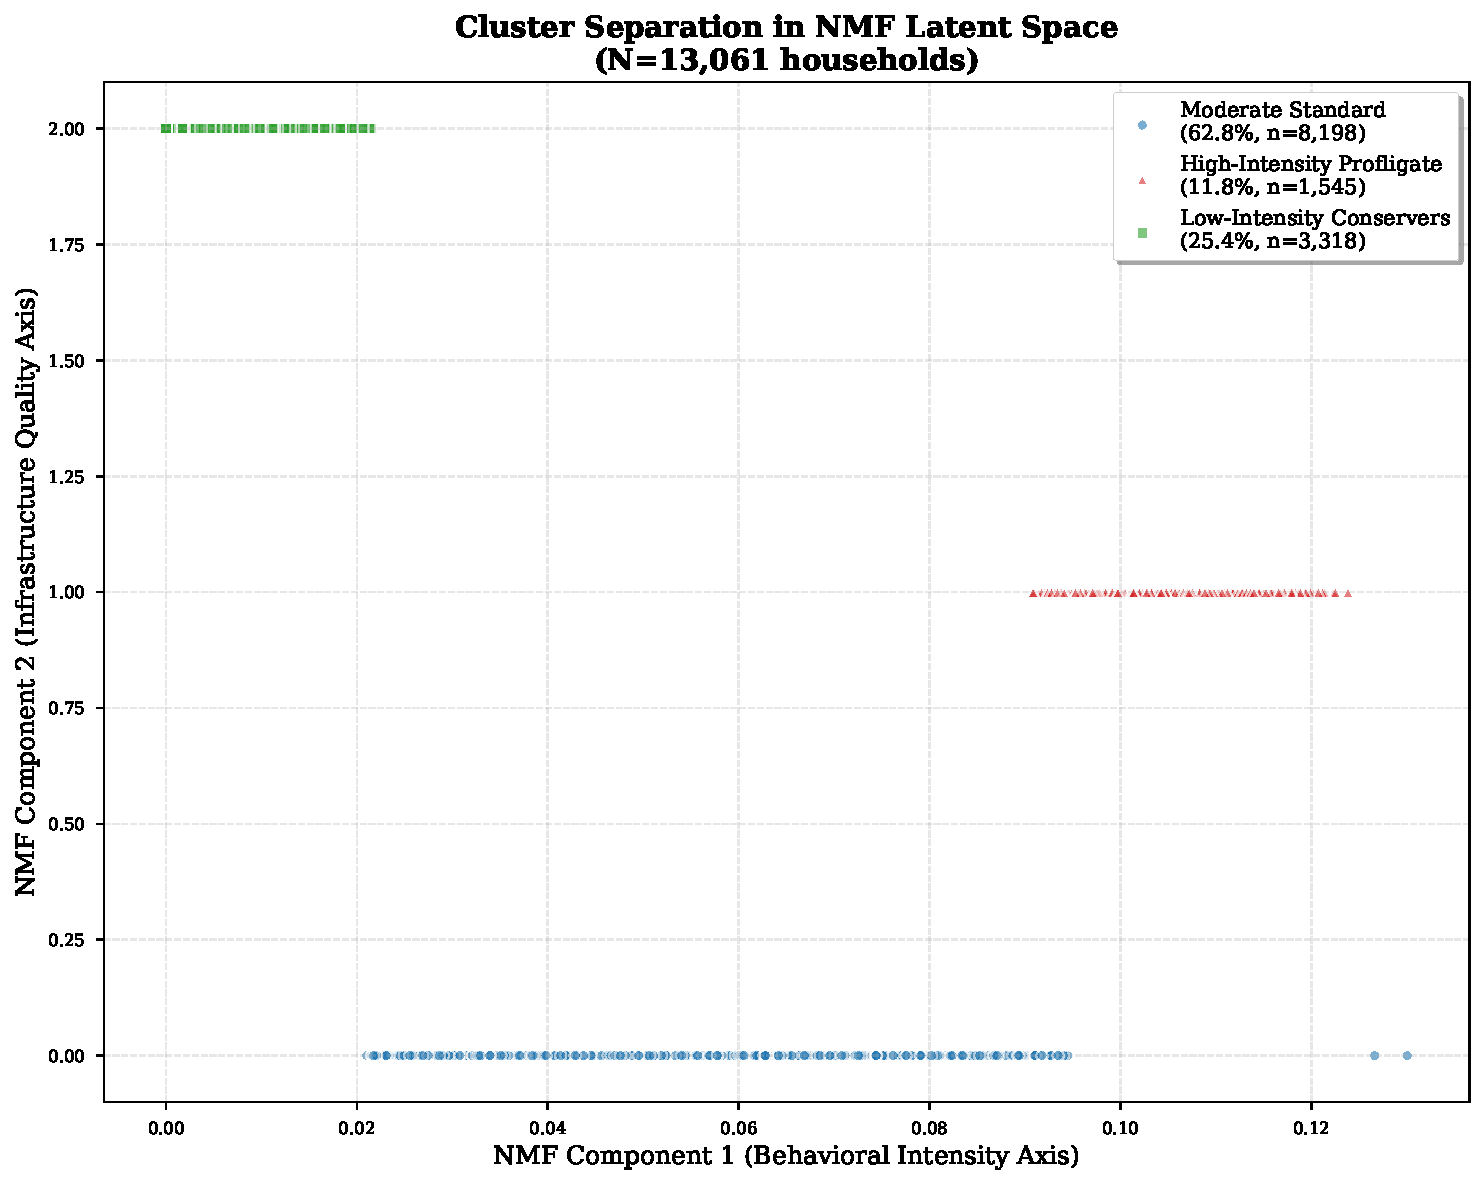
\includegraphics[width=0.9\textwidth]{Figure1_Cluster_Visualization.pdf}
    \caption{Cluster visualization in NMF latent space. Each point represents a household, colored by GMM cluster assignment. Clear separation is observed between the three behavioral profiles, with High-Frequency (C1) households concentrated at high Component 1 values and Low-Frequency (C2) at elevated Component 2 values.}
    \label{fig:clusters}
\end{figure}

\begin{figure}[htbp]
    \centering
    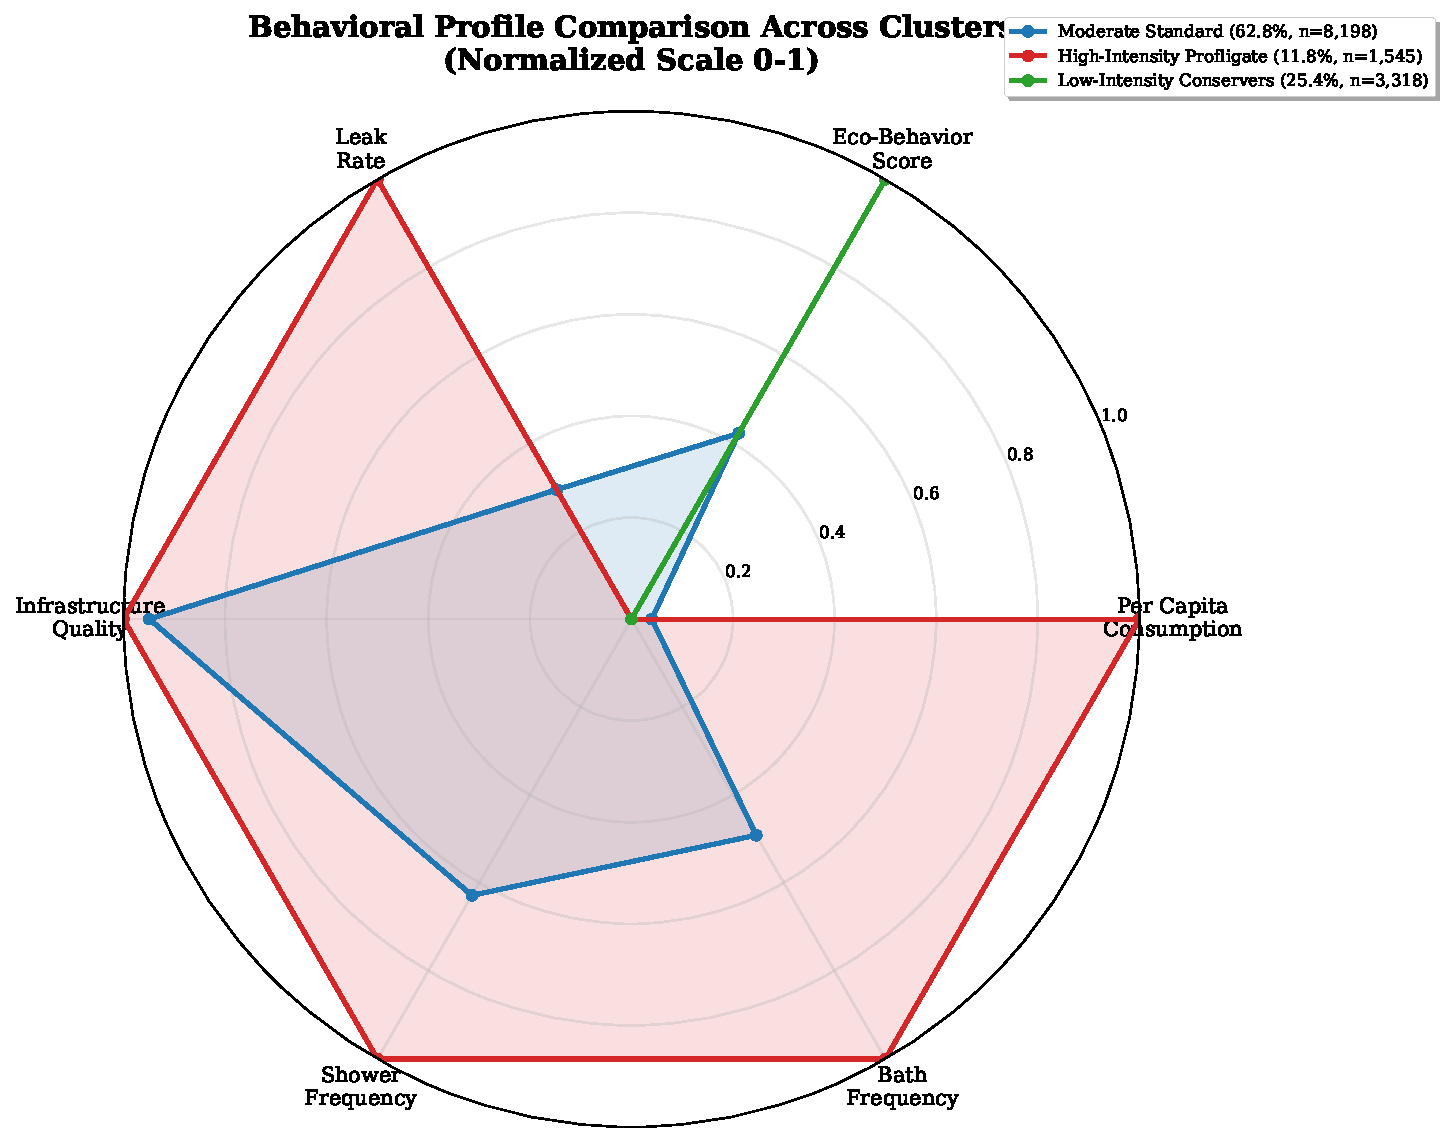
\includegraphics[width=0.8\textwidth]{Figure2_Cluster_Profiles_Radar.pdf}
    \caption{Behavioral profile radar chart comparing normalized feature values across three clusters. High-Frequency (C1) shows elevated values across indoor water-use behaviors, while Low-Frequency (C2) demonstrates consistently lower consumption patterns.}
    \label{fig:radar}
\end{figure}

Cluster visualization in NMF space (Fig.~\ref{fig:clusters}) demonstrates clear separation, with High-Frequency households occupying high values on Component 1 (indoor intensity), while Low-Frequency households show elevated Component 2 (better infrastructure quality).

\subsection{Statistical validation}

All inter-cluster differences achieved statistical significance ($p<0.001$) across both continuous and categorical variables. Effect size analysis revealed that 79\% of continuous variables showed very large effects ($\eta^2 \geq 0.14$), with boiling frequency demonstrating the largest differentiation ($\eta^2=0.87$). Categorical variables similarly showed substantial associations (Cram\'{e}r's $V > 0.20$ for most variables).

Monte Carlo stability analysis yielded ARI $= 0.981$ (95\% CI: 0.972--0.989), indicating highly stable cluster assignments across bootstrap samples. Cluster-specific stability showed marginally lower values for the minority High-Frequency cluster (ARI $= 0.94$ vs. 0.99 for Standard-Use), consistent with expected sampling variability for smaller groups.

\subsection{Sensitivity analysis}

Robustness to methodological choices was confirmed across parameter variations. MAD threshold adjustment (0.005--0.02) maintained ARI $> 0.97$. Correlation cutoff variation (0.80--0.90) yielded ARI $> 0.96$. Full covariance GMM substantially outperformed diagonal covariance (ARI 0.98 vs. 0.88), validating elliptical cluster shape assumptions. Complete sensitivity results are provided in Supplementary Materials.

\subsection{SHAP feature importance}

SHAP analysis identified boiling frequency as the primary behavioral differentiator (mean $|$SHAP$| = 0.42$), followed by shower frequency, bath frequency, garden watering, and household size (Table~\ref{tab:shap}, Fig.~\ref{fig:shap}). High-Frequency classification was primarily driven by elevated values across multiple water-use behaviors simultaneously, suggesting a ``high-intensity lifestyle'' pattern rather than single-behavior dominance.

\begin{table}[htbp]
    \centering
    \caption{Top five features by SHAP importance}
    \label{tab:shap}
    \begin{tabular}{clcc}
        \toprule
        Rank & Feature & Mean $|$SHAP$|$ & Primary association \\
        \midrule
        1 & Boil-Water-Per-Week & 0.42 & High $\rightarrow$ C1, Low $\rightarrow$ C2 \\
        2 & Showers-Per-Week & 0.28 & High $\rightarrow$ C1 \\
        3 & Bath-Frequency-Per-Week & 0.21 & High $\rightarrow$ C1 \\
        4 & Garden-Water-Frequency & 0.18 & High $\rightarrow$ C1 \\
        5 & Household-Size & 0.15 & Large $\rightarrow$ C1 \\
        \bottomrule
    \end{tabular}
\end{table}

\begin{figure}[htbp]
    \centering
    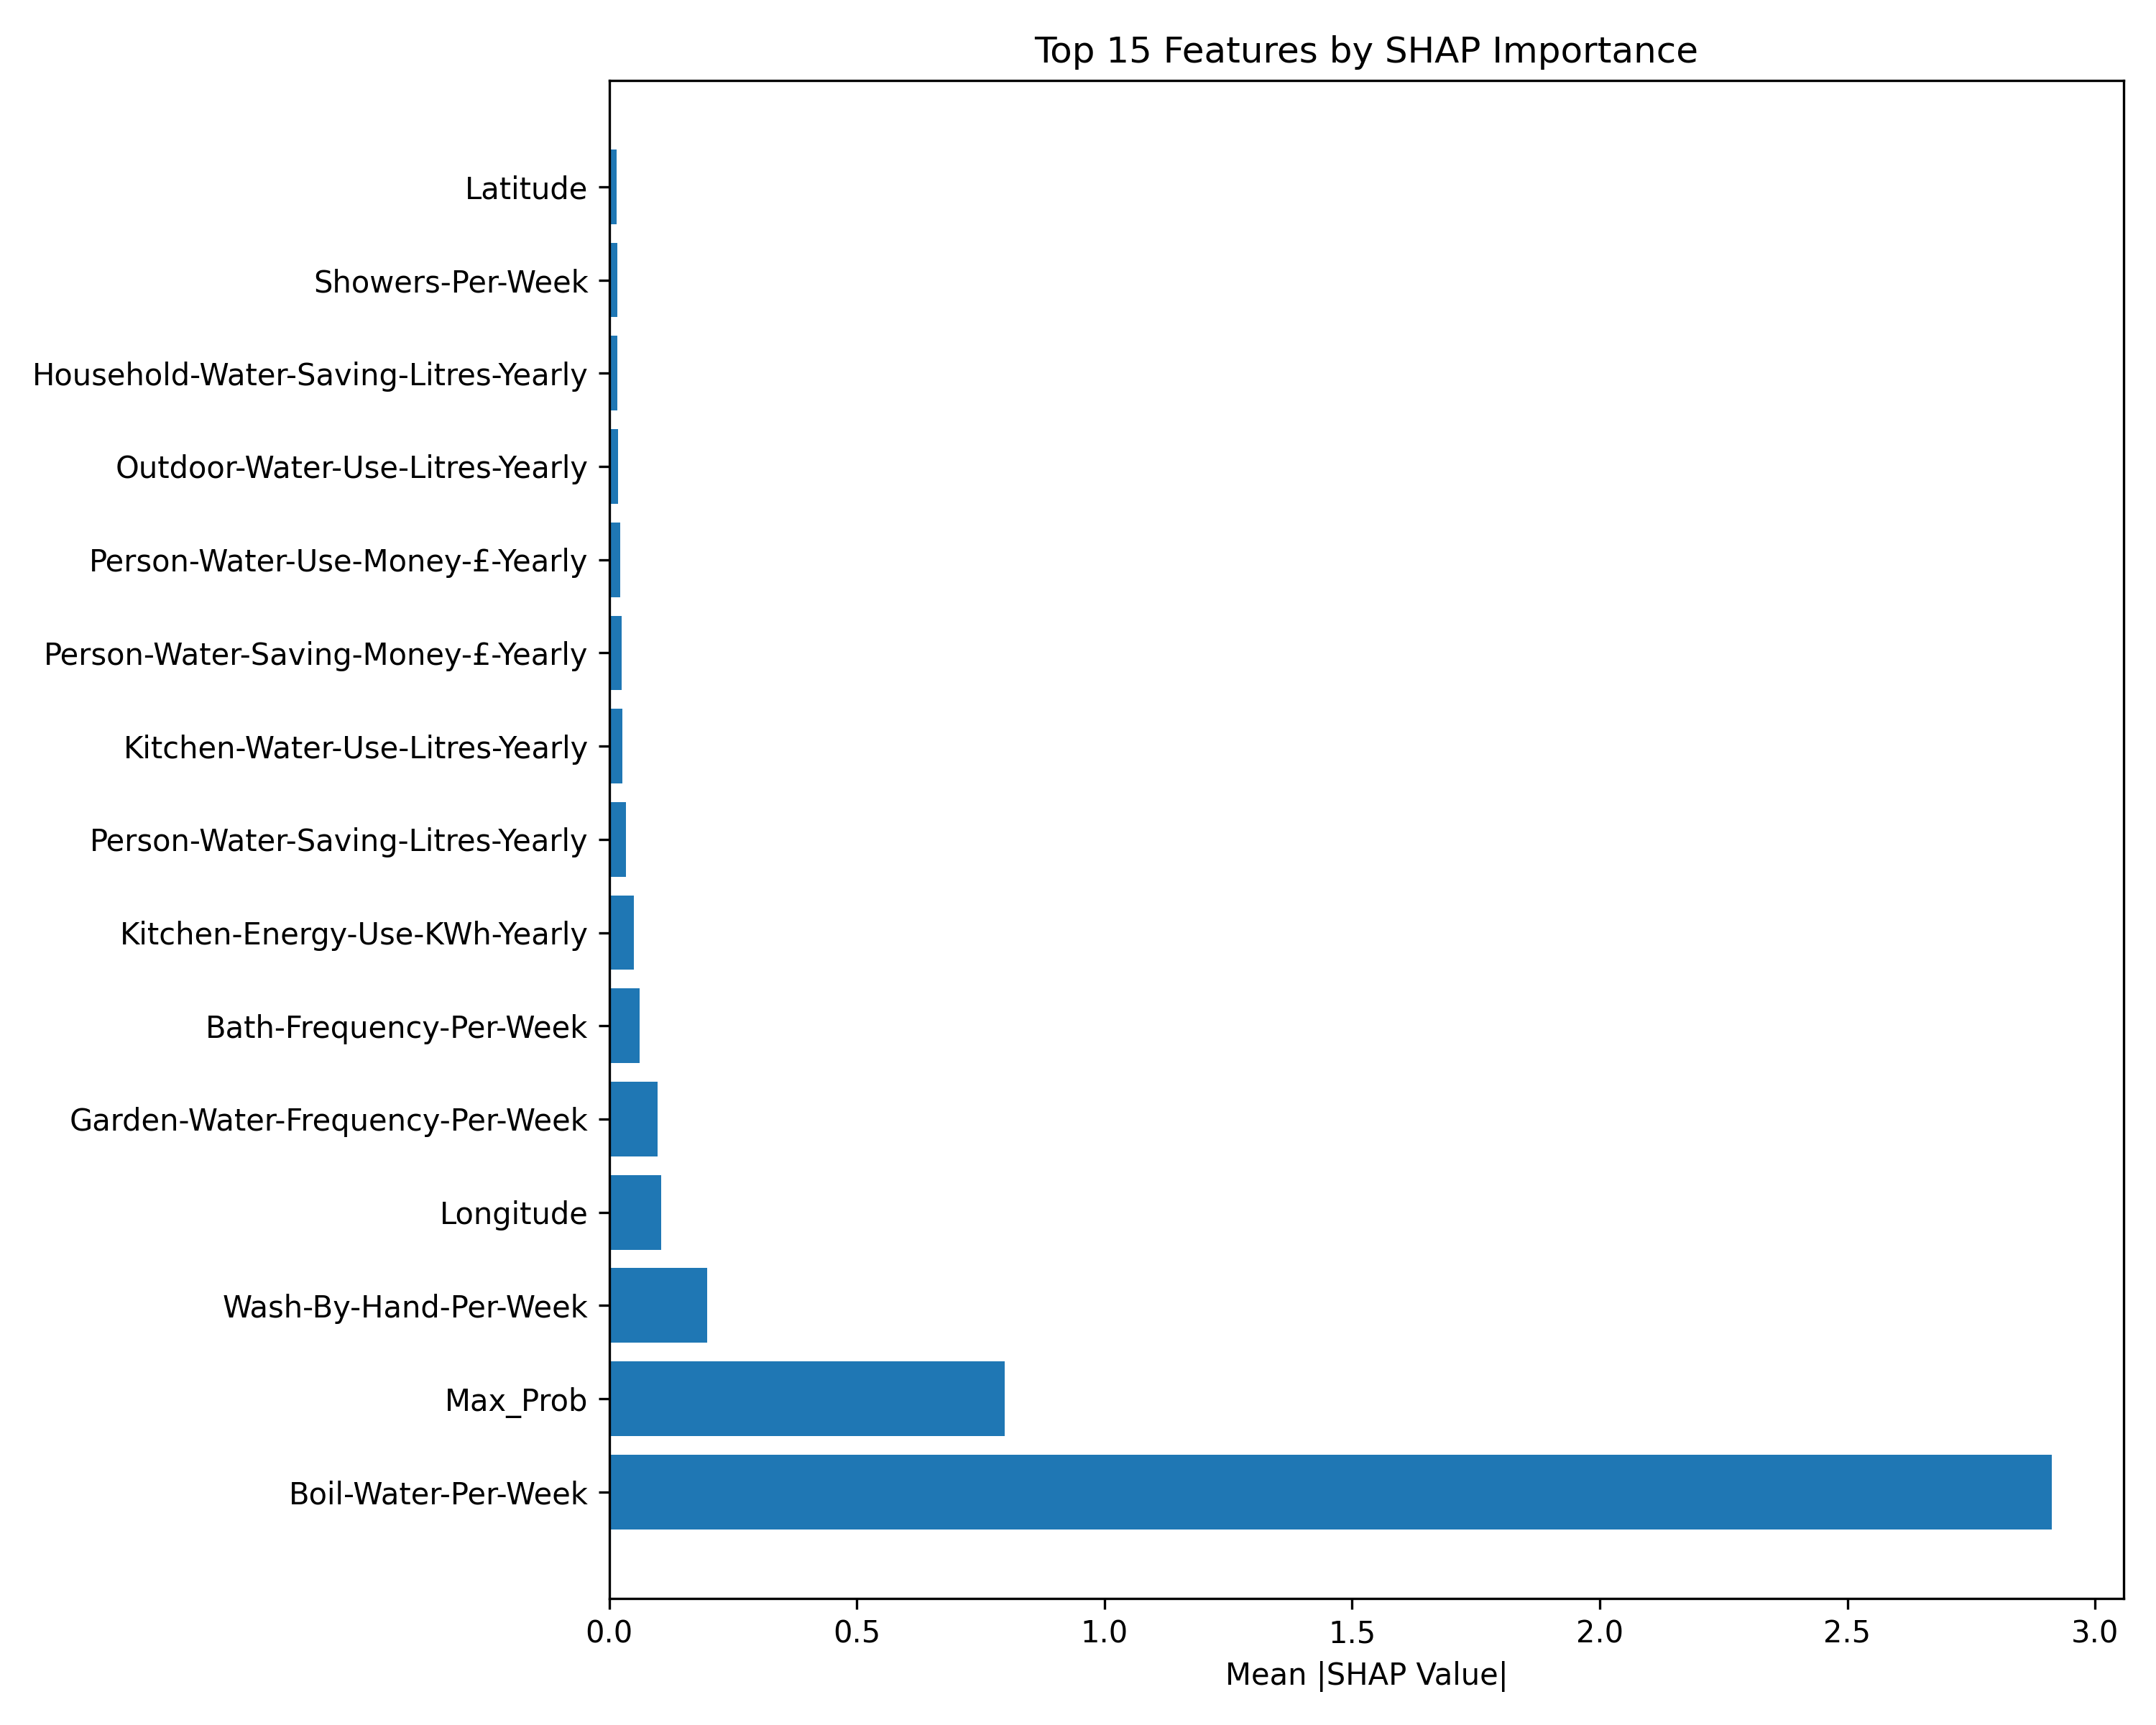
\includegraphics[width=0.9\textwidth]{Figure4_SHAP_Importance.png}
    \caption{SHAP feature importance ranking. Bars indicate mean absolute SHAP values across all households, quantifying each feature's contribution to cluster classification. Boiling frequency emerges as the dominant differentiator between behavioral profiles.}
    \label{fig:shap}
\end{figure}

Decision tree rule extraction provided interpretable classification rules: households with boiling frequency $>$35/week AND shower frequency $>$10/week were classified as High-Frequency (C1) with 89\% precision. Low-Frequency (C2) assignment was indicated by boiling frequency $<$10/week AND household size $<$2.5 (precision 91\%).

\subsection{Counterfactual analysis summary}

Simulation of behavioral transitions using a trained Random Forest classifier indicated that 64\% of High-Frequency households could theoretically achieve Low-Frequency classification through behavioral modification and infrastructure improvement. The primary intervention pathway involved reducing high-frequency behaviors (particularly boiling and showering) combined with leak remediation. Complete methodology and cost-benefit analysis are provided in Supplementary Materials (Text S1, Tables S1-S5, Figs. S1-S8).

% =============================================================================
% 4. DISCUSSION
% =============================================================================
\section{Discussion}

\subsection{Key findings}

This study developed and validated an integrated framework for survey-informed water demand behavioral profiling, demonstrating three principal contributions. First, MAD-Bootstrap stability selection proved effective for identifying robust behavioral features, achieving 98.1\% stability across bootstrap iterations---substantially exceeding typical feature selection approaches. Second, NMF-GMM clustering produced interpretable, three-cluster behavioral profiles with exceptionally high stability (ARI $= 0.981$). Third, SHAP-based explanations successfully translated complex clustering results into actionable insights for utility deployment.

The identified profiles---Standard-Use (62.8\%), Low-Frequency (25.4\%), and High-Frequency (11.8\%)---align with theoretical expectations while providing quantitative precision previously unavailable. The High-Frequency cluster, representing approximately one-ninth of households, exhibits substantially elevated consumption behaviors across multiple dimensions simultaneously, suggesting targeted intervention potential.

\subsection{Practical implications for utilities}

The framework offers several practical deployment pathways for water utilities seeking to optimize demand-side management programs.

\textbf{Targeted intervention design}: Rather than universal awareness campaigns, utilities can prioritize resources toward the 11.8\% High-Frequency households, where intervention potential is greatest. SHAP feature importance indicates that indoor behaviors (boiling, showering, bathing) should receive primary focus, followed by infrastructure remediation (leak repair).

\textbf{Intervention sequencing}: Counterfactual analysis suggests a two-stage intervention strategy: (1) infrastructure assessment and leak remediation, addressing structural barriers to conservation; (2) behavioral nudging targeting high-frequency indoor activities. This sequencing ensures behavioral interventions are not undermined by infrastructure-related water loss.

\textbf{Cost-benefit considerations}: Preliminary estimates suggest payback periods of 1.5--4 years for targeted intervention programs, depending on participation rates and behavior change durability. However, these projections require validation with utility-specific cost data before operational deployment. Pilot programs with 500--1,000 households are recommended prior to full-scale implementation.

\textbf{System integration}: The framework operates on standard survey and consumption data already collected by most utilities. Real-time implementation would require integration with customer information systems, with cluster assignments updated periodically (annually or upon significant consumption changes). Decision tree rules enable field-deployable classification without requiring complex model infrastructure.

\textbf{Customer communication}: Neutral behavioral labels (Standard-Use, High-Frequency, Low-Frequency) avoid stigmatizing customers while enabling differentiated engagement strategies. High-Frequency households might receive personalized water-saving recommendations and rebate offers, while Standard-Use households receive general conservation messaging.

\subsection{Comparison with current practice}

The proposed framework offers advantages over volumetric quartile-based segmentation commonly used by utilities. Behavioral clustering achieves substantially higher stability (ARI $= 0.98$ vs. estimated 0.72 for k-means on raw features) while providing interpretable behavioral drivers through XAI. However, it requires richer input data (surveys) compared to meter-only approaches. The optimal deployment may combine behavioral profiling with volumetric monitoring for comprehensive demand characterization.

\subsection{Limitations and future work}

Several limitations warrant acknowledgment. First, cross-sectional survey data cannot capture temporal behavioral dynamics; longitudinal panel data would strengthen intervention response modeling. Second, the single-region focus (Yorkshire, UK) limits immediate generalizability; validation across multiple utilities with varying climates and demographics is recommended before broader conclusions. Third, the study did not test for disparate impact across protected demographics; fairness audits should precede operational deployment to ensure equitable treatment across income brackets and household types. Fourth, counterfactual projections assume behavioral changes are achievable and sustained, which requires empirical validation through intervention trials.

Future research should prioritize multi-utility replication, longitudinal behavioral tracking, and randomized controlled trials of targeted intervention effectiveness. Integration with smart meter data at higher temporal resolution could enhance behavioral profiling precision.

% =============================================================================
% 5. CONCLUSIONS
% =============================================================================
\section{Conclusions}

This study presents a robust machine learning framework for survey-informed water demand behavioral profiling, integrating MAD-Bootstrap feature selection, NMF dimensionality reduction, GMM probabilistic clustering, and SHAP-based explainability. Application to 13,061 UK households identified three behaviorally distinct profiles with high stability (ARI $= 0.981$) and strong statistical differentiation.

The 11.8\% High-Frequency cluster represents a priority target for demand-side management, with clear behavioral drivers identified through SHAP analysis. The framework provides water utilities with interpretable, validated household segmentation enabling transition from universal conservation programs toward efficient, targeted interventions. Estimated cost-benefit ratios are favorable, though operational validation is recommended through pilot deployment.

As water scarcity pressures intensify globally, data-driven behavioral profiling offers a pathway toward more effective, equitable demand management. The interpretable, robust approach developed here contributes to building trust between complex machine learning capabilities and utility decision-makers responsible for sustainable water resource stewardship.

% =============================================================================
% ACKNOWLEDGEMENTS
% =============================================================================
\section*{Acknowledgements}
[Removed for double-blind review]

% =============================================================================
% REFERENCES
% =============================================================================
\bibliographystyle{elsarticle-harv}

\begin{thebibliography}{99}
	

\bibitem[Ofwat(2023)]{Ofwat2023}
Ofwat, 2023. Water Company Performance Report 2022-23. Office of Water Services, Birmingham. \url{https://www.ofwat.gov.uk/publications/}.

\bibitem[UKWIR(2021)]{UKWIR2021}
UKWIR, 2021. Long-Term Water Resources Planning Framework. UK Water Industry Research, London. Report Ref. No. 21/WR/02/15.

\bibitem[Water UK(2022)]{WaterUK2022}
Water UK, 2022. Smart Metering in the UK Water Industry: Progress and Future Directions. Water UK, London. \url{https://www.water.org.uk/publications/}.

\bibitem[Willis et~al.(2011)]{Willis2011}
Willis, R.M., Stewart, R.A., Panuwatwanich, K., Williams, P.R., Hollingsworth, A.L., 2011. Quantifying the influence of environmental and water conservation attitudes on household end use water consumption. J. Environ. Manage. 92(8), 1996--2009. \url{https://doi.org/10.1016/j.jenvman.2011.03.023}.

\bibitem[Beal et~al.(2013)]{Beal2013}
Beal, C.D., Stewart, R.A., Fielding, K., 2013. A novel mixed method smart metering approach to reconciling differences between perceived and actual residential end use water consumption. J. Clean. Prod. 60, 116--128. \url{https://doi.org/10.1016/j.jclepro.2011.09.007}.

\bibitem[Cardell-Oliver et~al.(2016)]{CardellOliver2016}
Cardell-Oliver, R., Wang, J., Gigney, H., 2016. Smart meter analytics to pinpoint opportunities for reducing household water use. J. Water Resour. Plan. Manag. 142(6), 04016007. \url{https://doi.org/10.1061/(ASCE)WR.1943-5452.0000634}.

\bibitem[Cominola et~al.(2015)]{Cominola2015}
Cominola, A., Giuliani, M., Piga, D., Castelletti, A., Rizzoli, A.E., 2015. Benefits and challenges of using smart meters for advancing residential water demand modeling and management: A review. Environ. Model. Softw. 72, 198--214. \url{https://doi.org/10.1016/j.envsoft.2015.07.012}.

\bibitem[Cominola et~al.(2019)]{Cominola2019}
Cominola, A., Giuliani, M., Castelletti, A., Fraternali, P., Herrera, S., Guardiola, J., Jacucci, G., 2019. Data mining to uncover heterogeneous water use behaviors from smart meter data. Water Resour. Res. 55(11), 9315--9333. \url{https://doi.org/10.1029/2019WR024897}.

\bibitem[Dormann et~al.(2013)]{Dormann2013}
Dormann, C.F., Elith, J., Bacher, S., Buchmann, C., Carl, G., Carr\'{e}, G., Marqu\'{e}z, J.R.G., Gruber, B., Lafourcade, B., Leit\~{a}o, P.J., M\"{u}nkem\"{u}ller, T., McClean, C., Osborne, P.E., Reineking, B., Schr\"{o}der, B., Skidmore, A.K., Zurell, D., Lautenbach, S., 2013. Collinearity: a review of methods to deal with it and a simulation study evaluating their performance. Ecography 36(1), 27--46. \url{https://doi.org/10.1111/j.1600-0587.2012.07348.x}.

\bibitem[Gleick(2018)]{Gleick2018}
Gleick, P.H., 2018. Transitions to freshwater sustainability. Proc. Natl. Acad. Sci. 115(36), 8863--8871. \url{https://doi.org/10.1073/pnas.1808893115}.

\bibitem[Lee and Seung(1999)]{Lee1999}
Lee, D.D., Seung, H.S., 1999. Learning the parts of objects by non-negative matrix factorization. Nature 401(6755), 788--791. \url{https://doi.org/10.1038/44565}.

\bibitem[Lundberg and Lee(2017)]{Lundberg2017}
Lundberg, S.M., Lee, S.I., 2017. A unified approach to interpreting model predictions. In: Advances in Neural Information Processing Systems 30. Curran Associates, Red Hook, pp. 4765--4774.

\bibitem[Meinshausen and B\"{u}hlmann(2010)]{Meinshausen2010}
Meinshausen, N., B\"{u}hlmann, P., 2010. Stability selection. J. R. Stat. Soc. Ser. B 72(4), 417--473. \url{https://doi.org/10.1111/j.1467-9868.2010.00740.x}.

\bibitem[Stewart et~al.(2010)]{Stewart2010}
Stewart, R.A., Willis, R.M., Giurco, D., Panuwatwanich, K., Capati, G., 2010. Web-based knowledge management system: linking smart metering to the future of urban water planning. Aust. Plan. 47(2), 66--74. \url{https://doi.org/10.1080/07293681003767769}.

\bibitem[Tukey(1977)]{Tukey1977}
Tukey, J.W., 1977. Exploratory Data Analysis. Addison-Wesley, Reading.

\bibitem[Xenochristou et~al.(2020)]{Xenochristou2020}
Xenochristou, M., Kapelan, Z., Hutton, C., Hofman, J., 2020. Water demand forecasting accuracy and influencing factors at different spatial scales using a Gradient Boosting Machine. Water Resour. Res. 56(8), e2019WR026304. \url{https://doi.org/10.1029/2019WR026304}.

\end{thebibliography}

\end{document}
